\section{State of The Art}
\label{sec:int_state}
\subsection{Infrared Thermography Techniques}
\par Starting by its discovery, infrared radiation was first reported by Hershel's famous experiment with a prism that would decompose the solar light. Frederick William Hershel noticed that when he placed a thermometer outside the visible spectrum, its temperature would still increase and deducted the existence of invisible radiation. The first patent of a radiation based thermometer was emitted in the end of the 19th century \cite{DeWitt1988}. Only after World War II a single point laser thermometer used in medicine, started being commercialized. Thermal cameras started being developed after the second World War, mainly for military purposes. A few years later IR systems would be used in various types of supersonic wind tunnels to detect aerodynamic heating. \\

%%% Czysz
\par In 1969, Czysz and Dixon \cite{Dixon1969} proposed a thermographic method to gather quantitative results. They applied a Phosphors coating to the surface. This coating is very sensitive to temperature. They placed heat sensors in key spots. The next step would be to use an Isodensitracer, a device that would read the density of the coating, make a density map (with iso-lines) and attribute a measured heat flux to each density level. They concluded stating that the key to gathering good quantitative results was to perform a good calibration. \\
%%% Sargent 
\par Inspired by Czysz and Dixon's work, in 1998, Sargent \textit{et al.} \cite{Sargent1998} followed the same approach and decided to use an IR camera to measure heat transfer in complex flows. Their calibration consisted in placing several thermocouples in their target surface. This calibration is often called \textit{in situ} calibration, for being made in the measured body. After collecting the video tape from the camera and post-processing it in the computer these authors correlated the grey scale values of the image with the temperatures measured by the sensors. The result can be seen in Figure \ref{fig:sargent}. This figure also shows the fitting curves, usually polynomials of second and third order. Czysz and Dixon \cite{Dixon1969} concluded that IR Cameras had a strong potential to be used in fluid dynamics measurements. They also concluded that \textit{in situ } calibrations can be very useful as they eliminate the need to calculate emissivity. \\

\begin{figure}
\centering
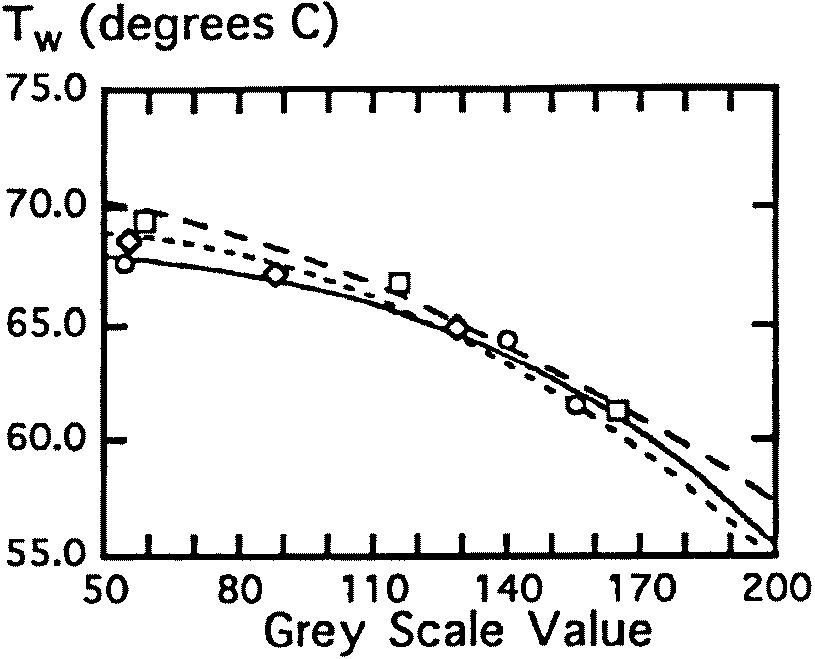
\includegraphics[width=0.5\linewidth]{Figures/1.Chapter/sargent.png}
\caption{Calibration of an IR Camera with polynomial fit}
\source{Sargent, 1998 \cite{Sargent1998}}
\label{fig:sargent} 
\end{figure}

%% Schwabe
\par In 2003, Schwabe \textit{et al.} \cite{schwabe2003oscillatory} pioneered the study of interfacial phenomena with an IR Camera. The experiments consisted on a cold surface where water would condensate, then flow back into a gap through a channel, where it would evaporate again. This was a closed cycle, covered by heated walls and a window made of Zinc Sulfide, a material transparent to IR radiation. To avoid condensation on the glass, a heater was placed on its center. However, this heater was a big obstruction to the camera's top view. \\

%%%Shen

\par In 2008, Shen \textit{et al.} \cite{shen2010simultaneous} studied simultaneous droplet impact and its influence on heat transfer from different heated surfaces. The used technique consisted in placing a high-speed camera horizontally to the droplet impact area and a infrared camera bellow the studied surface. They addressed the influence of surface topography on the heat transfer processes and observed that nano-structured surfaces had a significant lower heat removal by the droplets, when compared to smooth surfaces. It was also observed that the spreading diameter would increase with the surface heating for the nano-structured surface, while evaporation time was reduced.\\


%%Gerardi
\par In 2008, Gerardi \textit{et al.} \cite{Gerardi2008} started using thermographic cameras to study heat transfer through the macro- and micro-layer boiling applications. They wanted to observe bubble formation and study heat transfer in the interface between the bubble and the heated surface. Bubble formation is a phenomena that occurs between a small time window. To achieve this a IR Camera with high temporal resolution was used alongside with a high speed camera. The bubble formation was observed from the bottom of the experimental setup. This could only be done with a dichroic beamsplitter, that transmits IR radiation to the IR camera and is transparent to the visible light. To allow the radiation to pass from the bubble, the heated surface had to be transparent to both visible and infrared spectra, so it was made of sapphire. The sapphire thin plate had also a deposited film so it could be heated by Joule effect. With this setup it was possible to observe heat removal from a bubble from a constant heat flux source as it departs, with elevated time precision. The fact that Gerardi \textit{et al.} \cite{Gerardi2008} were able to synchronize the frames of both the IR and the high speed cameras enabled them to put side by side the images of both cameras. Correspondence of temperature maps and the phases of bubble departure was made so that thermal and physical phenomena could be matched. \\

%%Tartarini
\par In 2009, Tartarini \textit{et al.} \cite{tartarini2009} crossed the study of droplet cooling with infrared thermography. While previous studies focused mainly on stable isothermal conditions, Tartarini \textit{et al.} decided to focus on the study of transient conditions. To do this, the authors chose to use a IR transparent slab, heated by two radiators. Again, the IR camera would be put under the droplet, that would collect data, which would be processed in MATLAB to remove noise and apply an emissivity map. Tartarini \textit{et al.} coated the surface with a high emissivity paint on its upper side. This procedure aimed at minimizing errors associated to emissivity and study more accurately the solid-fluid interface. The experimental data allowed these authors validating a numerical model to predict transient temperatures. It was also possible to observe temperature drop at the center of the droplet using a time-frame of a minute. \\

%%Girard
\par In 2010, Girard \textit{et al.} \cite{girard2010infrared} used thermography in order to study droplet evaporation. In this experiment, like the one of Tartarini \textit{et al.} made, the author used an elevated time-frame, but with a more fine temporal resolution. In this setup a droplet fell on a heated copper surface. The IR camera was placed on top of the droplet on this setup. The authors observed the evaporation time using different surface temperatures. They focused on the interface between the water droplet and copper surface that due to their different emissivity was pretty noticeable. Based on this, Girard \textit{et. al.} reported the interface temperature and droplet radius along the time. \\

%% Kim and Buongiorno
\par In 2011, Kim and Buongiorno \cite{kim2011detection} proceeded with the work started in 2008 by Gerardi \textit{et al.} and used thermography to detect the triple interface between solid-liquid-vapour in pool boiling with a similar setup. To detect this interface they used an optical silicon wafer (transparent to IR) in contrast with \cite{Gerardi2008} which used coated sapphire. The camera detected the bubbles as dark spots and the liquid as bright spots. In this work the different absorptivity and temperatures of the distinct phases were used to detect the triple contact-line. Kim and Buongiorno observed the formation of a microlayer, where the radiation from the vapor would cross the water, and an area where the radiation would come from the bubble. The frontier between was concluded to be the limit between these 2 regions. \\

%% Duan
\par In 2013 Duan \textit{et al.} \cite{duan2013synchronized} synchronized not only the high-speed camera with the IR camera, but also used Particle Image Velocimetry (PIV) data. The objective was studying bubble formation and departure in pool boiling. The approach to use the IR camera was similar to \cite{Gerardi2008} but the high speed camera was placed horizontally to the boiling cell. Glass windows were mounted all around the wall to enable side view. The PIV laser was placed in the window frontal to the high speed camera's window. These authors could observe a dependence of the interval between bubble departure and formation with temperature, a strong cooling underneath the bubble, due to the microlayer. The observation of micro scale phenomena was only possible only by combining the high-speed camera, the IR camera and PIV. \\

%% Sielaf

\par More recently (2014), Sielaf \cite{sielaff2014experimental} used a different technique to gather interface data from pool boiling. Sielaf used a thin stainless steel foil under a heater. Given the small thickness of the foil, the interface temperature on top of the foil would be very close to that of the bottom surface. Sielaf also used a calibration technique close to the \textit{in situ} approach. With a thermocouple inside is pool boiling cell, near the foil and with the very close assumption that the foil would be at the same temperature, each pixel was calibrated for that temperature. Additional noise filters were applied in the post processing. As many of previously mentioned authors, Sielaf used the high-speed camera horizontally to his boiling cell. Another characteristic of his technique was that the foils enabled him to identify the transition from the contact line to a microlayer. Sielaf identified that this transition occurs during the receding phase of the bubble. \\

%% Zupancic
\par Additional studies using a thin foil have been performed in the past year. For instance, in 2015 Zupancic \textit{et al.} used this approach while also applying different coatings to study different wettability regimes. In this study, the heating of the foil is made directly by Joule effect with copper contacts on the foil. In 2016 Petkovsek \textit{et al.} observed, with a similar setup the hot spot phenomena. In this hot spot, measured temperature would be higher than the surroundings. \\

\subsection{Numerical Studies}

\par In this section some relevant numerical work about heat transfer in droplet impact will be discussed. This work contributed aswell to better understanding droplet related phenomena and heat transfer.\\
\par Numerous numerical droplet simulations have been performed in the last century, but the assumptions made to simplify them were questioned by several authors such as Healy \textit{et al.} \cite{healy2001validity} in 2001. Heat transfer during the spreading phase had been neglected, for representing a small fraction of the evaporation time. Although it seems a reasonable assumption, Healy \textit{et al.} found that in the spreading phase, the droplet temperature raise caused an alteration of its properties which resulted in significant errors. Still in 2001, Pasandideh-Fard \textit{et al.} \cite{pasandideh2001cooling} tested a numerical model that studied heat extraction, comparing it between impact velocities. Besides validating the model, impact velocity had a weak effect on the calculated temperature variation and heat flux. The principal effect of the increase of this parameter is that more area is wetted which means that extracts heat from a greater area. Later in 2010, Strotos \textit{et al.} \cite{strotos2011non} was able to identify, in his numerical work, various phenomena such as the bubble trapping effect and the neck in the droplet's lamela, and the heat transfer effects that these phenomena cause. In the case of the bubble trapping effect, an increase of the temperature in the droplet center, in the first moments after the impact was noted. In the case of the lamela neck a relation was made between its formation and position and an increase of temperature in that area.


